%====================================================
%	CHAPTER 4 - Control
%====================================================
\chapter{Controller Development}
\label{ch:control}
%====================================================
\section{Control Loop}
%====================================================
The control problem for this dissertation is, as outlined in Chater:\ref{ch:intro}; to achieve dynamic (\emph{attitude}) set point tracking on a quadrotor by solving the problem of its inherent underactuation. For the purposes of the subsequent controller development, the plant is described in the following non-linear state space form:
\begin{subequations}
\begin{equation}
\dot{\mathbf{x}}=f(\mathbf{x},t)+g(\mathbf{x},\vec{\nu},t)
\end{equation}
\vspace{-15pt}
\begin{equation}
y = c(\mathbf{x},t)+d(\mathbf{x},\vec{\nu},t)
\end{equation}
\end{subequations}
Where the plant dynamics are governed by $f(\mathbf{x},t)$ and the plant's input response by $g(\mathbf{x},\vec{\nu},t)$, for a given input $\vec{\nu}$. The latter is not necessarily a function based relationship and could take the multiplicative form; $g(\mathbf{x},t)\vec{\nu}$. The objective for setpoint tracking is for the output to track the state $y = \mathbf{x}$. As such, the control problem is to design a stabilizing control law for an error state $\mathbf{x}_e$\footnote{Ignoring how the state error is formulated for the time being\ldots}:
\\
\vspace{-5pt}
\begin{equation}
\vec{\nu}_d=h(\mathbf{x}_e,t)
\end{equation}
Such that the control plant is globally asymptotically stable or that $\lim_{t\rightarrow\infty}\mathbf{x}_e=0$. It is possible to combine attitude and position states into a common trajectory state such that:
\\
\vspace{-5pt}
\begin{equation}
\mathbf{x}=\begin{bmatrix}
\vec{\mathcal{E}}\\
Q_b
\end{bmatrix}
\end{equation}
The body's trajectory is then fully described by $\mathbf{x}(t)$. Separate control laws are developed for attitude and position tracking and hence those states aren't combined. However for the purposes of discussing the control plant, a single major loop is considered. The designed control input, $\vec{\nu}_d$, is then implemented by actuator suite $u\in\mathbb{U}$ through its effectiveness function:
\\
\vspace{-5pt}
\begin{equation}
\nu_c=B(\mathbf{x},u,t)
\end{equation}
The exact relationship of the virtual control input and commanded input, $\nu_c\rightarrow\nu_d$, is governed by the allocation algorithm. That allocation function, $B^\dagger$, can be \emph{roughly} referred to as the effectiveness inverse\footnote{Inversion (\emph{pseudo}) is the typical allocation scheme.}. The actuator positions are then solved, avoiding saturation, subject to some constraint as:
\begin{equation}
\underset{\in\mathbb{U}}{u}=B^{\dagger}(\mathbf{x},\nu_d,t)
\end{equation}
The control allocation requirements and schemes are expanded upon subsequently in Section:\ref{sec:control.allocation}. Multiple attitude controllers are presented whose stability is proven with Lyapunov$^\dagger$ stability theorem. Each controller is compared in the context of an over actuated quadrotor plant. Similarly a series of proposed allocation schemes are evaluated too. Those comparisons, their details and how controller efficacy and stability are evaluated is all presented next in Chapter:\ref{ch:simulation}. 
\newpage
A generalized over-actuated control loop is split into a series of cascaded control blocks, each with an individual function, as illustrated in Fig:\ref{fig:control-loop}. From the error state of the generated trajectory, $\mathbf{x}_e$, the control law designs a virtual control input, $\vec{\nu}_d$, which is cast as the argument to the allocation block. From the allocation law, $B^{\dagger}$, physical actuator positions are obtained; $u\in\mathbb{U}$. Those actuator positions effect a virtual plant input, $\vec{\nu}_c=B(\mathbf{x},u,t)$, which is an input to the state function's dynamics, Eq:\ref{eq:quaternion-states}. Not shown, but implied in Fig:\ref{fig:control-loop}, is the state derivative feedback of $\dot{\mathbf{x}}$ to the plant transfer function. Finally the output tracking state is estimated with some filtration paradigm, $\hat{\mathbf{x}}=A(\mathbf{x},t)$, and fed back to the error state.
\begin{figure}[htbp]
\centering
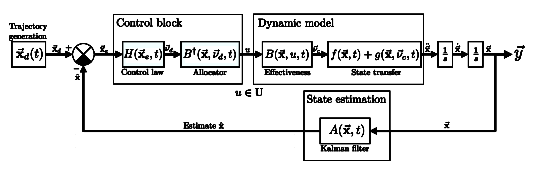
\includegraphics[width=0.95\textwidth]{figs/control-loop}
\caption{Generalized control loop with allocation}
\label{fig:control-loop}
\end{figure}
\vspace{-20pt}
%====================================================
\section{Control Plant Inputs}
\label{sec:control.inputs}
%====================================================
Thus far control plant inputs for the set of differential state equations, from Eq:\ref{eq:quaternion-states}, have mostly been described with net forces and torques; $\mu\vec{F}$ \& $\mu\vec{\tau}$. The relationship between each propeller's rotational speed \& servo positions and the its resultant output thrust direction is calculated as a quaternion transformation of produced lift force, as in Eq:\ref{eq:quaternion-inputs}.
\begin{subequations}\label{eq:control-input}
\begin{equation}
\mu\vec{F}(u)=\sum Q_{M_i}^*(\lambda_i,\alpha_i)\otimes T(\Omega_i)\otimes Q_{M_i}(\lambda_i,\alpha_i)~~~~\in\mathcal{F}^b
\end{equation}
\vspace{-10pt}
\begin{equation}
\mu\vec{\tau}(u)=\sum \vec{l}\times\big(Q_{M_i}^*(\lambda_i,\alpha_i)\otimes T(\Omega_i)\otimes Q_{M_i}(\lambda_i,\alpha_i)\big)~~~~\in\mathcal{F}^b
\end{equation}
\end{subequations}
To accommodate comparison of each controller and allocation scheme, the error state control law(s) design net plant inputs $\mu\vec{F}$ and $\mu\vec{\tau}$. The allocation rule then takes both net inputs as an argument to find actuator positions to effect those net inputs. As such each control law can be tested against various allocation rules and \emph{vise versa}. However typical allocation algorithms, like pseudo-inversion, require a multiplicative relationship between plant and control inputs\ldots 
\par
The actuator effectiveness functions in Eq:\ref{eq:control-input} aren't readily reducible to a single multiplicative relationship. Thusly the effectiveness function needs an extra layer of abstraction to incorporate a multiplicative relationship. Rather than calculating actuator positions directly from $\vec{\nu}_d$, a set of four 3-dimensional thrust vectors, $\vec{T}_{1\rightarrow 4}$, for each motor module are calculated first.
\begin{equation}\label{eq:4.7}
\vec{\nu}_d=\begin{bmatrix}
\mu\vec{F}\\
\mu\vec{\tau}
\end{bmatrix}
= 
\begin{bmatrix}
1 & 1 & 1 & 1\\
\vec{l}_\times & \vec{l}_\times & \vec{l}_\times & \vec{l}_\times
\end{bmatrix}
\begin{bmatrix}
\vec{T}_1\\
\vec{T}_2\\
\vec{T}_3\\
\vec{T}_4
\end{bmatrix}
\end{equation}
Where $\vec{l}_\times$ is the cross product vector of the torque arm. Individual actuator positions for each module, $[\Omega,~\lambda,~\alpha]^T$, can be calculated from those thrust vectors $\vec{T}_i$ for $i\in[1:4]$ with some trigonometry, ensuring that they only adhere to Eq:\ref{eq:control-input}. That trigonometric inversion\footnote{Inverting either rotation matrix operations or quaternions to solve for angular servo positions.} can be described as the function $R^\dagger$:
\begin{equation}\label{eq:4.8}
[\Omega_i,~\lambda_i,~\alpha_i]^T=R^\dagger(\mathbf{x},\vec{F}_i,t)~~~~i\in[1:4]
\end{equation}
\par
To summarize then; each allocation rule controls designs net thrust vectors for each of the four modules, or 12 directional components, in the following form:
\begin{equation}
B^{\dagger}(\mathbf{x},\vec{\nu}_d,t)=\big[ T_{1x},~T_{1y},~T_{1z},~\ldots~T_{4x},~T_{4y},~T_{4z}\big]^T
\end{equation}
The control block in the loop (Fig:\ref{fig:control-loop}) is then modified to incorporate the extra abstraction level, shown in Fig:\ref{fig:control-block}. The output from that control block is still the same actuator matrix $u\in\mathbb{U}$. The block merely accommodates for comparison of various $B^\dagger$ allocation rules without compromising the entire loop's structure.
\begin{figure}[htbp]
\centering
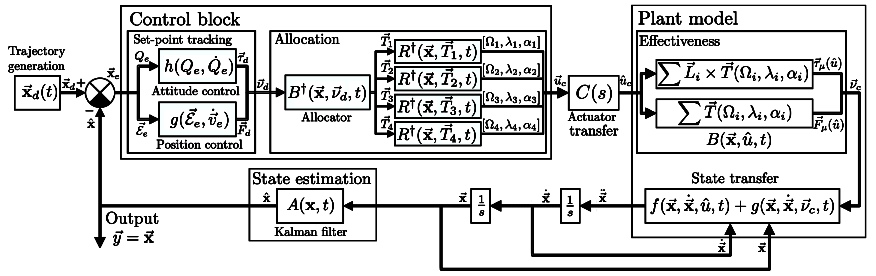
\includegraphics[width=0.67\textwidth]{figs/control-block}
\caption{Abstracted control block}
\label{fig:control-block}
\end{figure}
\par
\vspace{-10pt}
\emph{\color{Gray} Al allocation algorithms proposed follow the same input/output structure described in Fig:\ref{fig:control-block}. Only one allocation algorithm does, however, circumvent the virtual abstraction level of thrust vector's for each module to directly calculate actuator positions, Section:\ref{subsec:control.allocation.online}.}
\par
Each control law is co-dependent on an accompanying allocation algorithm. Traditional control loops (under-actuated or well matched) typically have a unity allocation algorithm and as such require no consideration so they're mostly disregarded. Separate control laws for attitude ad position control are presented next in Section:\ref{sec:control.attitude} and \ref{sec:control.position} respectively. Thereafter a series of allocation rules are proposed in Section:\ref{sec:control.allocation}. Although presented independently, the controller and allocation laws are mutually inclusive. The stability of each control law is proven objectively but actual controller tuning and optimization takes place only in the next chapter in Section:\ref{sec:simulation.tuning}.
\par
%====================================================
\subsection*{Model Dependent \& Independent Controllers}
%====================================================
Two classes of controllers are presented, attitude and position control laws. The former being the primary focus of this research project and containing a more verbose control treatment. Both control categories consider MIMO state vector loops for $\mathcal{E}$ \& $Q_b$. The allocation algorithm combines both virtual control inputs $\vec{\mu}_d=[\mu\vec{F}~\mu\vec{\tau}]^T$ generated from the two control categories to calculate actuator positions.
\par
The control dependency on the system plant is as a consequence of the prominent actuator response dynamics, as derived previously in Section:\ref{subsec:dynamics.nonlinearities.gyrotorques} from Chapter:\ref{ch:dynamics}. Whilst not a prerequisite for stability, plant dependent compensation certainly improves controller performances. Independent and dependent cases are only presented in one type of controller; the most basic case PD controller in Section:\ref{subsec:control.attitude.controllers}. It's shown that for an independent (\emph{PD}) controller to achieve global stability some stringent assumptions must  be met.
\par
Inherent plant dependency makes backstepping controllers an attractive control paradigm in this dissertation's context. The proposed dependent control laws compensate for undesirable dynamics their design, basic PD \& PID control structures (\emph{and the like}) will not. The first and most basic control solution, used as a reference case, is a PD controller for attitude and position with direct-inversion\footnote{Pseudo-inversion or Moore-Penrose inversion} allocation, both plant dependent and independent controllers are compared.
%====================================================
\section{Lyapunov Stability Theorem}
\label{sec:control.lyapunov}
%====================================================
Lyapunov's stability theory is a critical aspect of non-linear controller design. An abundance of literature has been written on the subject\footnote{included in almost every meritable textbook and papers \cite{noteonlyapunov,nonlinearsystems} amongst others\ldots} spanning through the progression of control engineering. Typically linear systems are proven$^\dagger$ to be stable in the frequency domain, the same is not true for non-linear systems. Lyapunov's stability theorem proves (\emph{global}) asymptotic stability for continuous time invariant systems, linear or otherwise.
\par
The theorem applies analysis of a generalized energy function representative of a system's autonomous trajectory. A negative energy derivative will ensure the system's energy is always dissipating toward a stable settling point. Lyapunov analysis is a popular method for stability verification because the trajectory of the system needn't be explicitly defined for stability to be ascertained. Proof of Lyapunov's theorem is done with a contradiction disproof and, as such, the theoretical underpinning is somewhat cumbersome.
\par
Despite the conceptually difficult proof, it's worth reiterating its fundamentals given that backstepping controllers are proposed later in Section:\ref{subsec:control.attitude.nonlinear} for attitude control. A backstepping controller iteratively enforces Lyapunov stability criterion onto the system through the control structure. In general, given a non-linear time invariant system that follows some continually differentiable trajectory $\mathbf{x}(t)$, typically the trajectory is going to progress subject to some rule:
\begin{equation}
\dot{\mathbf{x}}(t)=f\big(\mathbf{x}(t)\big)
\end{equation}
Then, constructing a generalized positive definite function (a generalized energy or \emph{Lyapunov candidate} function) $V(x)$ for a trajectory $x=\mathbf{x}(t)$. A positive definite matrix, $M$, is defined such that $z^TMz\geq 0~\forall z$. As such an LCF typically has the form:
\begin{equation}
V=x^TPx
\end{equation}
Given that by definition the trajectory is continually differentiable, there is a gradient matrix for $V(x)$ in the form:
\begin{equation}
\nabla V(x)=\bigg[\frac{\delta V(x)}{\delta x_1}~\frac{\delta V(x)}{\delta x_2}~\ldots~\frac{\delta V(x)}{\delta x_n}\bigg]~~~~x\in\mathbb{R}^n
\end{equation}
The energy function's derivative, otherwise refereed to as the \emph{Lie derivative}$^\dagger$, is calculated as follows:
\begin{equation}
\dot{V}(x)=\nabla V(x)^Tf(x)=\frac{\delta V(x)}{\delta x_1}f_1(x)+~\ldots~+\frac{\delta V(x)}{\delta x_n}f_n(x)
\end{equation}
Lyapunov's theorem states that \emph{iff} the candidate function $V(x)$ is positive definite with $\dot{V}(0)=0$ and its derivative is negative definite; $\dot{V}(x)< 0~~\forall z \not= 0$, the system is then globally asymptotically stable. Mathematically that means, for any $\mathbf{x}(t)\geq 0$:
\begin{equation}
V\big(\mathbf{x}(t)\big)=V\big(\mathbf{x}(0)\big)+\int_0^t \dot{V}\big(\mathbf{x}(t)\big).dt \leq V\big(\mathbf{x}(t)\big)
\end{equation}
Which can be physically interpreted as the system's generalized energy function always dissipating, irrespective of trajectory path taken. With a continually decreasing energy, the system will eventually settle to some stable point, hence the trajectory exists in some bounded $\big\{x|V(x)\leq V\big(\mathbf{x}(t)\big)\big\}$, which is defined as global asymptotic stability. Every trajectory of $\dot{\mathbf{x}}(t)=f\big(\mathbf{x}(t)\big)$ converges to the zero\footnote{adapted to zero error state tracking} setpoint as $t\rightarrow\infty$.
\par
The asymptotic stability proof can be extended to exponential stability boundedness, such that the same conditions are met and there is some positive $\alpha>0$ such that $\dot{V}(x)\leq-\alpha V(x)$. That implies the system is globally exponentially stable as is bound in such a manner that:
\begin{equation}
||\mathbf{x}(t)||\leq Me^{-\alpha t/2}||\mathbf{x}(0)||
\end{equation}
%====================================================
\section{Attitude Control}
\label{sec:control.attitude}
%====================================================
\subsection{The Attitude Control Problem}
\label{subsec:control.attitude.problem}
%====================================================
Set point tracking control of the attitude plant is to then design a stabilizing control torque $\mu\vec{\tau}=h(\mathbf{x}_e,t)$ such that; for any desired attitude quaternion, $\forall~Q_d\in\mathbb{Q}$, and an instantaneous attitude body quaternion, similarly $\forall~Q_b\in\mathbb{Q}$, the error state asymptotically stabilizes; $Q_e\rightarrow[1~\vec{0}~]^T$. Or that:
\begin{equation}
\mu\vec{\tau}=h(Q_e,~\dot{Q}_e)~~\text{such that}~~\underset{t\rightarrow\infty}{\lim}Q_e=\begin{bmatrix}
1\\
\vec{0}
\end{bmatrix}
\end{equation}
Quaternion error states are defined as the Hamilton product (\emph{difference}) between the desired and current quaternion attitudes. Quaternion error states are in contrast with the subtractive relationship for Euler angle error states. The attitude error state is calculated as:
\begin{equation}\label{eq:quaternion-error}
Q_e=Q_d^*\otimes Q_b
\end{equation}
The relative angular velocity between the body frame, $\mathcal{F}^b$, and the trajectory's desired frame, $\mathcal{F}^d$, is given as $\vec{\omega}_e$. The body angular velocity, $\vec{\omega}_b$ is subject to the differential Eq:\ref{eq:quaternion-states-angular}. As such there's an angular rate error:
\begin{subequations}
\begin{equation}\label{eq:angular-error}
\vec{\omega}_e=\vec{\omega}_d-\vec{\omega}_b
\end{equation}
The desired angular rate is taken with respect to the desired angular attitude frame, and so it must be transformed to the existing body frame.
\begin{equation}
\vec{\omega}_e=Q_e^*\otimes\vec{\omega}_d\otimes Q_e-\vec{\omega}_b
\end{equation}
Typically, for the trajectories generated here, $\vec{\omega}_d=\vec{0}$ so the angular rate error is simply the negative body angular velocity. It would be easy to include a non-zero angular velocity setpoint.
\begin{equation}
\vec{\omega}_e=-\vec{\omega}_b
\end{equation}
\end{subequations}
The time derivative of the quaternion error state is then, dependent on the angular velocity error, given as:
\begin{equation}
\dot{Q}_e=\frac{1}{2}Q_e\otimes\vec{\omega}_e=-\frac{1}{2}Q_e\otimes\vec{\omega}_b
\end{equation}
%====================================================
\subsection{Linear Controllers}
\label{subsec:control.attitude.controllers}
%====================================================
\subsubsection{PD Controller}
\label{subsubsec:control.attitude.controllers.pd}
%====================================================
The control law which is used as a basic reference for comparison is a simple Proportional-Derivative structured attitude controller. Specifically, a stability proof derived from the one presented \emph{The Attitude Control Problem}\cite{attitudecontrolproblem} is used for asymptotic stability verification. An attitude PD control law, proportional to quaternion error and angular rate error, designs the control torque as:
\begin{equation}\label{eq:independent-pd}
\mu\vec{\tau}_{_{PD}}=K\vec{\omega}_e+\alpha\vec{q}_e
\end{equation}
Where both $K$ and $a$ are positive definite $3\times 3$ coefficient matrices still to be determined. This control law does not take into account the quaternion error scalar. Then using a candidate Lyapunov energy function $V_{_{PD}}$:
\begin{equation}\label{eq:lyapunov-pd}
V_{_{PD}}=\alpha\vec{q}_e^{~T}\vec{q}_e+\alpha(q_0-1)^2+\frac{1}{2}\vec{\omega}_e^{~T}\mathbb{I}_b\vec{\omega}_e
\end{equation}
And recalling from Eq:\ref{eq:quaternion-states-angular} that body's the angular velocity differential $\dot{\vec{\omega}}_b$ is:
\begin{equation}
\dot{\vec{\omega}}_b=\mathbb{I}_b^{-1}\big(-\vec{\omega}_b\times\mathbb{I}_b\vec{\omega}_b+\vec{\tau}_Q+\vec{\tau}_g+\vec{Q}+\mu\vec{\tau}\big)
\end{equation}
With actuator inputs $u\in\mathbb{U}$ implied and $\vec{Q}$ being a simplified representation of the net aerodynamic torque experienced by the body from the rotating propellers, drawn from Eq:\ref{eq:aerodynamic-torque}. Then, noting that from quaternion's inherent properties, it follows that:
\begin{equation}\label{eq:4.17}
\vec{q}^{~T}\vec{q}+q_0^2=\vec{q}^{~2}+q_0^2=1
\end{equation}
Substituting the angular velocity error state, $\vec{\omega}_e=-\vec{\omega}_b$, the proportional derivative LCF in Eq:\ref{eq:lyapunov-pd} is simplified\footnote{The quaternion scalar $q_0$ in Eq:\ref{eq:4.18} is implied to be the quaternion error scalar} to:
\begin{subequations}\label{eq:4.18}
\begin{equation}
V_{_{PD}}=\alpha\vec{q}_e^{~2}+\alpha q_0^2 -2q_0 + 1 +\frac{1}{2}\vec{\omega}_e^{~T}\mathbb{I}_b\vec{\omega}_e
\end{equation}
\vspace{-10pt}
\begin{equation}
=2\alpha(1-q_0)+\frac{1}{2}\vec{\omega}_b^{~T}\mathbb{I}_b\vec{\omega}_b
\end{equation}
\end{subequations}
Similarly, using the fact that for a quaternion's time derivative:
\begin{equation}\label{eq:quat-derivative}
\dot{Q}=\begin{bmatrix}
-\frac{1}{2}\vec{q}^{~T}\vec{\omega}\\
\frac{1}{2}\big(\vec{q}_\times+q_0\mathbb{I}\big)\vec{\omega}
\end{bmatrix}
\end{equation}
Then, resolving the above into the derivative of the LCF, $\dot{V}_{_{PD}}$:
\begin{subequations}
\begin{equation}
\dot{V}_{_{PD}}=2\alpha\frac{1}{2}\vec{q}_e^{~T}\vec{\omega}_e+\frac{1}{2}\dot{\vec{\omega}}_b^{~T}\mathbb{I}_b\vec{\omega}_b+\frac{1}{2}\vec{\omega}_b\mathbb{I}_b\dot{\vec{\omega}}_b^{~T}
\end{equation}
\vspace{-12pt}
\begin{equation}
-\alpha\vec{q}_e^{~T}\vec{\omega}_b+\vec{\omega}_b^{~T}\mathbb{I}_b\dot{\vec{\omega}}_b
\end{equation}
\end{subequations}
Simplifying the angular acceleration $\dot{\vec{\omega}}_b$ and introducing the PD control law, $\mu\vec{\tau}_{_{PD}}$:
\begin{subequations}
\begin{equation}
\vec{\omega}_b^{~T}\mathbb{I}_b\dot{\vec{\omega}}_b=\vec{\omega}_b^{~T}\big(-\vec{\omega}_b\times\mathbb{I}_b\vec{\omega}_b+\vec{\tau}_Q+\vec{\tau}_g+\vec{Q}-K\vec{\omega}_b+\alpha\vec{q}_e\big)
\end{equation}
\vspace{-12pt}
\begin{equation}
\dot{V}_{_{PD}}=-\alpha\vec{q}_e^{~T}\vec{\omega}_b+\vec{\omega}_b^{~T}\big(-\vec{\omega}_b\times\mathbb{I}_b\vec{\omega}_b+\vec{\tau}_Q+\vec{\tau}_g+\vec{Q}-K\vec{\omega}_b+\alpha\vec{q}_e\big)
\end{equation}
\end{subequations}
Then, under specific circumstances the following assumptions can be made to ensure asymptotic stability. The stability does break down if any of the assumptions fail, as such the stability is not global\ldots
\vspace{-10pt}
\begin{enumerate}[itemsep=0em]
\item The inertial matrix, $\mathbb{I}_b$, is roughly diagonal and that the angular rate is small, then:\\
$\vec{\omega}_b^{~T}\big(\vec{\omega}_b\times\mathbb{I}_b\vec{\omega}_b\big)\approx\vec{0}$
\item Similarly, because the actuator rate torque response, $\vec{\tau}_Q$, is a second order effect mostly dependent on $\dot{u}$. Typically the actuator rates are going to be small so any of the inertial responses to those position changes are small enough to be considered negligible. The approximation is made:\\
$\vec{\tau}_Q\approx\vec{0}$
\item Finally, for the sake of the stability proof, the eccentric gravitational torque arm is neglected, $\vec{\tau}_g\approx\vec{0}$. Such a situation only holds true if $u\approx\vec{0}$ or that servo actuator positions\footnote{Excluding propeller rotational speeds, considering only the servo positions} are close to their zero positions.
\end{enumerate}
{\emph{\color{Gray}All of these assumptions are made under extraneous circumstances and can't be assumed for almost all of the prototype's flight envelope. The plant independent case is considered and simulated purely for contrition; mainly to demonstrate the need for plant dependent compensation. All subsequent control laws compensate for the plant dynamic response torques introduced in Section:\ref{sec:dynamics.nonlinearities}.}
\par
If each of the assumptions made hold true, then the Lyapunov energy functions derivative is approximately negative definite.
\begin{subequations}
\begin{equation}
\dot{V}_{_{PD}}\approx-\alpha\vec{q}_e^{~T}\vec{\omega}_b+\vec{\omega}_b^{~T}\big(-K\vec{\omega}_b+\alpha\vec{q}_e\big)
\end{equation}
\vspace{-10pt}
\begin{equation}
\Rightarrow\dot{V}_{_{PD}}=-\vec{\omega}_b^{~T}K\vec{\omega}_b=-K||\vec{\omega}_b||^2\leq \vec{0}~~~~\forall~\mathbf{Z}(t)
\end{equation}
\end{subequations}
Where $\mathbf{Z}(t)$ is the generalized trajectory which includes $\vec{\omega}_b$ \& $Q_b$ and K is a positive (\emph{definite}) 3X3 coefficient matrix. Then from Lyapunov stability theorem\cite{.} the limits are; $\lim_{t\rightarrow\infty}\vec{\omega}_e=\vec{0}$, $\lim_{t\rightarrow\infty}\vec{q}_e=0$ and $\lim_{t\rightarrow\infty}(1-q_0)=0$. 
\newpage
Hence $Q_e\rightarrow[1~\vec{0}$\hspace{2pt}$]^{T}$ as $t\rightarrow\infty$, asymptotic stabilizing the attitude error state. Introducing model dependency compensation to the PD control law alleviates the stringent requirements on assumptions 1 through 3. 
\begin{equation}\label{eq:dependent-pd}
\mu\vec{\tau}_{_{PD}}=\vec{\omega}_b\times\mathbb{I}_b\vec{\omega}_b-\vec{\tau}_Q-\vec{\tau}_g-\vec{Q}+K\vec{\omega}_b+\alpha\vec{q}_e
\end{equation}
The resultant stability proof is for Eq:\ref{eq:dependent-pd} is much the same as for the independent Eq:\ref{eq:independent-pd} using the same LCF from Eq:\ref{eq:lyapunov-pd}. The resultant control law is less reliant on assumptions for stability to be achieved. The dynamic compensation in Eq:\ref{eq:dependent-pd} improves control response, especially considering the form of unwanted dynamics are already quantified previously and modelled with \emph{relative} confidence.
%====================================================
\subsubsection{Auxiliary Plant Controller}
\label{subsubsec:control.attitude.controllers.auxpd}
%====================================================
Expanding on what has, in practice, proven\footnote{Practical examples of various quadrotor attitude PD controllers listed in Table:\ref{tab:controllers}} to be a very popular and effective control law for attitude stabilization, McGilvray et al. [2006]\cite{attitudestabilization} suggested introducing an auxiliary plant term to a Proportional-Derivative structure. Their altered PD controller adds auxiliary terms proportional to the quaternion time derivative error, as part of the auxiliary plant is a term for the quaternion scalar. The scalar term is otherwise neglected in the previous PD control law (Section:\ref{subsubsec:control.attitude.controllers.pd}).
\par
The modified (\emph{auxilliarly}) PD control torque is designed dependent on errors states for quaternions, angular rates and quaternion rates.
\begin{equation}\label{eq:control-aux-pd}
\mu\vec{\tau}_{_{XPD}}=\underbrace{-\Gamma_2{\widetilde{\Omega}}-\Gamma_3\vec{q}_e+\mathbb{I}_b\dot{\bar{\Omega}}}_{Independent}+\underbrace{\vec{\omega}_b\times\mathbb{I}_b\vec{\omega}_b+\vec{\tau}_Q+\vec{\tau}_g+\vec{Q}}_{Compensation}
\end{equation}
In which case the coefficients\footnote{Reiterating that exact coefficient values are determined in Chapter:\ref{ch:simulation}\ldots} $\Gamma_2$ \& $\Gamma_3$ are both diagonal positive definite coefficient matrices and $\Gamma_1$, introduced subsequently, is a positive symmetric matrix. The auxiliary plants $\widetilde{\Omega}$ \& $\dot{\bar{\Omega}}$ are defined as follows, and drawing on Eq:\ref{eq:quat-derivative} for definition of some aspects. For the first auxiliary plant $\bar{\Omega}$ is proportional to the quaternion error and hence $\dot{\bar{\Omega}}$ is a quaternion derivative term:
\begin{subequations}\label{eq:aux-pd-1}
\begin{equation}
\bar{\Omega}=-\Gamma_1\vec{q}_e \rightarrow\dot{\bar{\Omega}}=-\Gamma_1\dot{\vec{q}}_e
\end{equation}
\vspace{-15pt}
\begin{equation}
\dot{\bar{\Omega}}=-\frac{1}{2}\Gamma_1\big(q_0\mathbb{I}_{3X3}+[\vec{q}_e]_{\times}\big)\vec{\omega}_e
\end{equation}
\vspace{-10pt}
\begin{equation}
=\frac{1}{2}\Gamma_1\big(q_0\mathbb{I}_{3X3}+[\vec{q}_e]_{\times}\big)\vec{\omega}_b
\end{equation}
\end{subequations}
And the second auxiliary plant, $\widetilde{\Omega}$, is a term proportional to a combined quaternion and angular velocity error state.
\begin{subequations}\label{eq:aux-pd-2}
\begin{equation}
\widetilde{\Omega}=\vec{\omega}_e-\bar{\Omega}=\vec{\omega}_e+\Gamma_1\vec{q}_e
\end{equation}
\vspace{-15pt}
\begin{equation}
=-\vec{\omega}_b+\Gamma_1\vec{q}_e
\end{equation}
\end{subequations}
Using an LCF similar to the basic one $V_{_{PD}}$ from Eq:\ref{eq:lyapunov-pd}, but introducing an auxiliary term $\widetilde{\Omega}$ into the candidate function $V_{_{XPD}}$:
\begin{equation}\label{eq:lyapunov-xpd}
V_{_{XPD}}=\vec{q}_e^{~T}\vec{q}_e+\big(q_0-1\big)^2+\frac{1}{2}\widetilde{\Omega}^{~T}\big(\Gamma3^{-1}\mathbb{I}_b\big)\widetilde{\Omega}
\end{equation}
Again using the simplification from a quaternion's inherent properties in Eq:\ref{eq:4.17}. Eq:\ref{eq:lyapunov-xpd} then simplifies to:
\begin{subequations}
\begin{equation}
V_{_{XPD}}=2(1-q_0)+\frac{1}{2}\widetilde{\Omega}^{~T}\big(\Gamma_3^{-1}\mathbb{I}_b\big)\widetilde{\Omega}
\end{equation}
\vspace{-10pt}
\begin{equation}
\dot{V}_{_{XPD}}=2\frac{1}{2}\vec{q}_e^{~T}\vec{\omega}_e+\frac{1}{2}{\dot{\widetilde{\Omega}}}\text{}^{~T}\big(\Gamma_3\mathbb{I}_b\big)\widetilde{\Omega}+\frac{1}{2}\widetilde{\Omega}\big(\Gamma_3\mathbb{I}_b\big)\dot{\widetilde{\Omega}}
\end{equation}
\vspace{-10pt}
\begin{equation}
\dot{V}_{_{XPD}}=-\vec{q}_e^{~T}\vec{\omega}_b+\frac{1}{2}\dot{\widetilde{\Omega}}\text{}^{T}\big(\Gamma_3\mathbb{I}_b\big)\widetilde{\Omega}+\frac{1}{2}\widetilde{\Omega}^T\big(\Gamma_3\mathbb{I}_b\big)\dot{\widetilde{\Omega}}
\end{equation}
\end{subequations}
It then follows from Eq:\ref{eq:aux-pd-2}:
\begin{subequations}
\begin{equation}
\dot{\widetilde{\Omega}}=-\dot{\vec{\omega}}_b+\Gamma_1\dot{\bar{\Omega}}\Rightarrow\dot{\vec{\omega}}_b=\mathbb{I}_b^{-1}\big(-\vec{\omega}_b\times\mathbb{I}_b\vec{\omega}_b+\vec{\tau}_Q+\vec{\tau}_g+\vec{Q}+\mu\vec{\tau}\big)
\end{equation}
\vspace{-15pt}
\begin{equation}
\therefore\dot{\widetilde{\Omega}}=-\mathbb{I}_b^{-1}\big(-\vec{\omega}_b\times\mathbb{I}_b\vec{\omega}_b+\vec{\tau}_Q+\vec{\tau}_g+\vec{Q}+\mu\vec{\tau}\big)-\Gamma_1\dot{\bar{\Omega}}
\end{equation}
Introducing the control law $\mu\vec{\tau}_{_{XPD}}$, Eq:\ref{eq:control-aux-pd}, to the auxiliary plant derivative.
\begin{equation}
\rightarrow\dot{\widetilde{\Omega}}=\mathbb{I}_b^{-1}\big(\mathbb{I}_b\dot{\bar{\Omega}}-\Gamma_2\widetilde{\Omega}-\Gamma_3\vec{q}_e\big)-\dot{\bar{\Omega}}
\end{equation}
\vspace{-15pt}
\begin{equation}
=\mathbb{I}_b^{-1}\big(\Gamma_2\widetilde{\Omega}-\Gamma_3\vec{q}_e\big)
\end{equation}
\end{subequations}
From the positive symmetric (or \emph{diagonal}) properties of the coefficient matrices $\Gamma_1$,$\Gamma_2$ \& $\Gamma_3$, then the auxiliary plant's transpose is:
\begin{equation}
\dot{\widetilde{\Omega}}\text{}^{T}=\mathbb{I}_b^{-1}\big(-\Gamma_2\widetilde{\Omega}^T-\Gamma_3\vec{q}_e\big)
\end{equation}
It then follows:
\begin{subequations}
\begin{equation}
\frac{1}{2}\dot{\widetilde{\Omega}}\text{}^{T}\big(\Gamma_3^{-1}\mathbb{I}_b\big)\widetilde{\Omega}=\frac{1}{2}\big(-\Gamma_2\widetilde{\Omega}^T-\Gamma_3\vec{q}_e^{~T}\big)\Gamma_3^{-1}\widetilde{\Omega}
\end{equation}
\vspace{-10pt}
\begin{equation}
=\frac{1}{2}\big(-\widetilde{\Omega}^T\Gamma_2\Gamma_3\text{}^{-1}\widetilde{\Omega}-\vec{q}_e\text{}^{T}\widetilde{\Omega}\big)
\end{equation}
And substituting Eq:\ref{eq:aux-pd-2}, $\vec{q}_e\text{}^T\widetilde{\Omega}=-\vec{q}_e\text{}^T\vec{\omega}_b+\Gamma_1\vec{q}_e\text{}^T$:
\begin{equation}
\frac{1}{2}\big(-\widetilde{\Omega}\text{}^T\Gamma_2\Gamma_3\text{}^{-1}\widetilde{\Omega}+\vec{q}_e\text{}^T\vec{\omega}_b-\vec{q}_e\text{}^T\Gamma_1\vec{q}_e\big)
\end{equation}
Similarly, for the transposed energy function counterpart:
\begin{equation}
\frac{1}{2}\widetilde{\Omega}\text{}^{T}\big(\Gamma_3\text{}^{-1}\mathbb{I}_b\big)\dot{\widetilde{\Omega}}=\frac{1}{2}\big(-\widetilde{\Omega}\Gamma_2\Gamma_3\text{}^{-1}\widetilde{\Omega}\text{}^T+\vec{q}_e\text{}^T\vec{\omega}_b-\vec{q}_e\Gamma_1\vec{q}_e\text{}^T\big)
\end{equation}
\end{subequations}
\vspace{-10pt}
\begin{equation}
\Rightarrow\dot{V}_{_{XPD}}=-\widetilde{\Omega}\Gamma_2\Gamma_3\text{}^{-1}\widetilde{\Omega}\text{}^T-\vec{q}_e\text{}^T\Gamma_1\vec{q}_e\leq\vec{0}~~~~\forall~(\widetilde{\Omega},\vec{q}_e)
\end{equation}
As such, the control law $\mu\vec{\tau}_{_{XPD}}$ asymptomatically stabilizes the attitude plant. Both $\widetilde{\Omega}$ and $\vec{q}_e$ tends to $\vec{0}$, or more specifically:
\begin{subequations}
\begin{equation}
\underset{t\rightarrow\infty}{\lim}\vec{q}_e=0
\end{equation}
\vspace{-10pt}
\begin{equation}
\underset{t\rightarrow\infty}{\lim}\widetilde{\Omega}=0
\end{equation}
Then, from the auxiliary plant definition in Eq:\ref{eq:aux-pd-2}, the following limits present themselves;
\begin{equation}
\underset{t\rightarrow\infty}{\lim}\vec{\omega}_b=0~~~\text{and}~~~\underset{t\rightarrow\infty}{\lim}\bar{\Omega}=0
\end{equation}
\end{subequations}
The stability proof for $V_{_{XPD}}$ can then be extended to true exponential stability. Exploiting the fact that $0\leq q_0 \leq 1$ it follows that:
\begin{equation}\label{eq:4.34}
1-q_0\leq 1-q_0^2=||\vec{q}_e||^2
\end{equation}
Seeing that exponential stability is a maximal boundedness proof, then the relationship Eq:\ref{eq:4.34} can replace the quaternion scalar term $2(1-q_e)$ in $V_{_{XPD}}$. For the stability proof the LCF is rewritten in terms of its norm(s):
\begin{subequations}\label{eq:xpd-ibc}
\begin{equation}
V_{_{XPD}}=\vec{q}_e\text{}^T\vec{q}_e+(q_0-1)^2+\frac{1}{2}\widetilde{\Omega}\text{}^T\big(\Gamma_3\text{}^{-1}\mathbb{I}_b\big)\widetilde{\Omega}
\end{equation}
\vspace{-10pt}
\begin{equation}
\leq 2||\vec{q}_e||^2+\frac{1}{2}\Gamma_3\text{}^{-1}\mathbb{I}_b||\widetilde{\Omega}||^2
\end{equation}
Similarly the LCF derivative can be written as:
\begin{equation}
\dot{V}_{_{XPD}}=-\Gamma_2\Gamma_3\text{}^{-1}||\widetilde{\Omega}||^2-\Gamma_1||\vec{q}_e||^2
\end{equation}
\end{subequations}
$V_{_{XPD}}$ then gains a maximum such that:
\begin{equation}
V_{_{XPD}}\leq max \bigg\{ 2,\frac{\lambda_{max}(\Gamma_3\text{}^{-1}\mathbb{I}_b)}{2}\bigg\}\big(||\vec{q}_e||^2+||\widetilde{\Omega}||^2\big)
\end{equation}
With $\lambda_{max}$ represents the maximum eigenvalue of $\Gamma_3\text{}^{-1}\mathbb{I}_b$. Similarly the \emph{negative definite} LCF derivative is bound by the minimum:
\begin{equation}
\dot{V}_{_{XPD}} \leq -min \big\{ \lambda_{min}(\Gamma_1),\lambda_{min}(\Gamma_2\Gamma_3\text{}^{-1})\big\}\big( || \vec{q}_e||^2+||\widetilde{\Omega}||^2 \big)
\end{equation}
Therefore there exists some ration $\beta$ that satisfies the relationship between the LCF and its derivative; $\dot{V}_{_{XPD}}\leq -\beta V_{_{XPD}}$, where $\beta$ is defined as:
\begin{equation}
\beta=\frac{min\big\{\lambda_{min}(\Gamma_1),\lambda_{min}(\Gamma_2\Gamma_3\text{}^{-1})\big\}-\big(||\vec{q}_e||^2+|||\widetilde{\Omega}||^2\big)}{max\big\{2,\frac{\lambda_{max}(\Gamma_3\text{}^{-1}\mathbb{I}_b)}{2}\big\}}
\end{equation}
The attitude trajectory $\big(\vec{q}_e(t),\widetilde{\Omega}(t)\big)$ is then exponentially bound:
\begin{equation}
\big(||\vec{q}_e(t)||,||\widetilde{\Omega}(t)||\big)\leq Me^{-\beta t/2}\big(||\vec{q}_e(0)||,||\widetilde{\Omega}(0)||\big)
\end{equation}
\emph{\color{Gray}The stability proof for the auxiliary attitude controller was expanded upon and derived from McGilvray et al. [2006]\cite{attitudestabilization} and adapted to fit attitude setpoint tracking. The fact that the auxiliary plant controller introduces the quaternion error, which is dependent on the quaternion scalar, greatly improves performance. The exponential stability notably improves settling, seen next in Chapter:\ref{ch:simulation}.}
\par
An earlier paper by Joshi, et al. [1995]\cite{robustattitude} was the precursor for PD based attitude plants with exponential stability. The control law first proposed didn't make use of any defined auxiliary plants, unlike \cite{attitudestabilization}, but equivalent terms were effectively incorporated. That control law developed for spacecraft attitude tracking proposed a very similar control scheme to $\mu\vec{\tau}_{_{XPD}}$. That controller, when changed to familiar notation used above, designs body torque as:
\begin{equation}
\mu\vec{\tau}^{\hspace{2pt}'}_{_{XPD}}=-\frac{1}{2}\bigg[\big([\vec{q}_e]_\times+q_0\mathbb{I}_{3X3}\big)\Gamma_1+\alpha\big(1-q_0\mathbb{I}\big)\bigg]\vec{q}_e-\Gamma_2\vec{\omega}_b
\end{equation} 
%====================================================
\subsubsection{PID Controller}
%====================================================
\emph{\color{Red}NEEDS WORK, POSSIBLY UNNECESSARY}
\par
Building on the previous two linear plant \emph{attitude} controllers, the final linear control structure proposed is arguably the most common control paradigm. 
\newpage
%====================================================
\subsection{Non-linear Controllers}
\label{subsec:control.attitude.nonlinear}
%====================================================
Backstepping controllers(\cite{satellitebackstepping,intelligentbackstep,backstepslidingmode} ,etc\ldots) are a popular choice for non-linear attitude plant control. The process iteratively enforces Lyapunov stability criteria to ensure asymptotic stability. In a report \cite{backstepping} Van Kampen, et al. [2008] describes fundamental backstepping algorithms. Ideal backstepping control is a precise control solution which requires exact plant matching, something that is difficult to achieve in practice. IBC control laws are especially susceptible to disturbances. The backstepping algorithm can then be extended to incorporate disturbance and uncertainty (\emph{estimate error}) terms, which are included in the LCF energy function. By Lyapunov's theorem those error terms are driven to 0.
%====================================================
\subsubsection{Ideal Backstepping Controller}
\label{subsubsec:control.attitude.nonlinear.idealbackstep}
%====================================================
Beginning with the ideal case for the first proposed backstepping controller, it's assumed the attitude plant described in Eq:\ref{eq:quaternion-states-angular}, from the consolidated model in Section:\ref{sec:dynamics.model}, is precise. The ideal backstepping controller aims to compensate for the plants dynamic response to trajectory inputs. Ignoring any uncertainty associated with the dynamic equation, the aim here is for a stabilizing torque design. Recalling the quaternion tracking error from Eq:\ref{eq:quaternion-error}; $Q_e=Q_d^*\otimes Q_b$. Then considering the first LCF:
\begin{equation}
V_1(\vec{q}_e)=\vec{q}_e\text{}^T\vec{q}_e+(q_0-1)^2
\end{equation}
Which, after substituting quaternion derivatives, has a Lie derivative:
\begin{subequations}
\begin{equation}
\dot{V}_1=2\vec{q}_e\text{}^T\dot{\vec{q}}_e+2(q_0-1)\dot{q}_0
\end{equation}
\vspace{-10pt}
\begin{equation}
=2\vec{q}_e\text{}^T\frac{1}{2}\big([\vec{q}_e]_\times+q_0\mathbb{I}_{3X3}\big)\vec{\omega}_e-2\big(q_0-1\big)\frac{1}{2}\vec{q}_e\text{}^T\vec{\omega}_e
\end{equation}
\vspace{-5pt}
\begin{equation}
=\vec{q}_e\text{}^T\big([\vec{q}_e]_\times+q_0\mathbb{I}_{3X3}\big)\vec{\omega}_e-q_0\vec{q}_e\text{}^T\vec{\omega}_e+\vec{q}_e\text{}^T\vec{\omega}_e
\end{equation}
\vspace{-8pt}
\begin{equation}
=\vec{q}_e\text{}^T[\vec{q}_e]_\times\vec{\omega}_e+\vec{q}_e\text{}^T\vec{\omega}_e
\end{equation}
\vspace{-8pt}
\begin{equation}
=-\vec{q}_e\text{}^T[\vec{q}_e]_\times\vec{\omega}_b-\vec{q}_e\text{}^T\vec{\omega}_b
\end{equation}
\end{subequations}
Then choosing the first stabilizing function $z_1$ with a virtual backstepping control input $\Omega_d$. It's important to note $\Omega_d$ is used here to differentiate the backstepping designed value and the trajectory instructed $\vec{\omega}_d$ from Eq:\ref{eq:angular-error}, or any auxiliary plants defined previously in Section:\ref{subsubsec:control.attitude.controllers.auxpd}.
\begin{equation}
\Omega_d=\Gamma_1\vec{q}_e
\end{equation}
Where $\Gamma_1$ is a symmetric positive definite coefficient matrix, a fact that is important to stress due to positive definite matrix's invertability. That stabilizing law then simplifies the LCF derivative $\dot{V}_1$ to:
\begin{subequations}
\begin{equation}
\dot{V}_1=-\vec{q}_e\text{}^T[\vec{q}_e]_\times\Gamma_1\vec{q}_e-\vec{q}_e\text{}^T\Gamma_1\vec{q}_e
\end{equation}
\vspace{-15pt}
\begin{equation}
=-\vec{q}_e\text{}^T\Gamma_1\vec{q}_e
\end{equation}
\end{subequations}
Where the virtual plant input creates an error
\begin{subequations}
\begin{equation}
z_1=\vec{\omega}_b-\Omega_d=\vec{\omega}_b-\Gamma_1\vec{q}_e
\end{equation}
\vspace{-15pt}
\begin{equation}
\rightarrow \vec{\omega}_b=z_1-\Gamma_1\vec{q}_e
\end{equation}
\end{subequations}
Introducing that error $z_1$ into a second LCF built from the first:
\begin{subequations}
\begin{equation}
V_2(\vec{q}_e,~z_1)=V_1(\vec{q}_e)+\frac{1}{2}z_1\text{}^T\Gamma_1\text{}^{-1}z_1
\end{equation}
\vspace{-10pt}
\begin{equation}
=\vec{q}_e\text{}^T\vec{q}_e+(q_0-1)^2+\frac{1}{2}z_1\text{}^T\Gamma_1\text{}^{-1}z_1
\end{equation}
\end{subequations}
That first error $z_1$ has its own derivative, recalling $\dot{\vec{\omega}}_b$ from earlier with an as yet undefined controllable input $\mu\vec{\tau}$:
\begin{subequations}
\begin{equation}
\dot{z}_1=\dot{\vec{\omega}}_b-\Gamma_1\dot{\vec{q}}_e
\end{equation}
\vspace{-10pt}
\begin{equation}
=\dot{\vec{\omega}}_b-\frac{\Gamma_1}{2}\big([\vec{q}_e]_\times+q_0\mathbb{I}_{3X3}\big)\vec{\omega}_b
\end{equation}
\vspace{-10pt}
\begin{equation}\label{eq:z-deriv}
=\mathbb{I}_b\text{}^{-1}\big(-\vec{\omega}_b\times\mathbb{I}_b\vec{\omega}_b+\vec{\tau}_Q+\vec{\tau}_g+\vec{Q}+\mu\vec{\tau}\big)-\frac{\Gamma_1}{2}\big([\vec{q}_e]_\times+q_0\mathbb{I}_{3X3}\big)\vec{\omega}_b
\end{equation}
\end{subequations}
So then, following from Eq:\ref{eq:z-deriv}, finding the derivative $\dot{V}_2$:
\begin{subequations}\label{eq:ibc-deriv}
\begin{multline}
\dot{V}_2(\vec{q}_e,~z_1)=\vec{q}_e\text{}^T\big(z_1-\Gamma_1\vec{q}_e\big)+z_1\text{}^T\Gamma_1\text{}^{-1}\bigg(\mathbb{I}_b\text{}^{-1}\big(-\vec{\omega}_b\times\mathbb{I}_b\vec{\omega}_b+\vec{\tau}_Q+\vec{\tau}_g+\vec{Q}+\mu\vec{\tau}\big)\\-\frac{\Gamma_1}{2}\big([\vec{q}_e]_\times+q_0\mathbb{I}_{3X3}\big)\vec{\omega}_b\bigg)
\end{multline}
\vspace{-20pt}
\begin{multline}
=-\vec{q}_e\text{}^T\Gamma_1\vec{q}_e+z_1\text{}^T\Gamma_1\text{}^{-1}\bigg(\Gamma_1\vec{q}_e+\mathbb{I}_b\text{}^{-1}\big(\vec{\omega}_b\times\mathbb{I}_b\vec{\omega}_b+\vec{\tau}_Q+\vec{\tau}_g+\vec{Q}+\mu\vec{\tau}\big)\\-\frac{\Gamma_1}{2}\big([\vec{q}_e]_\times+q_0\mathbb{I}_{3X3}\big)\vec{\omega}_b\bigg)
\end{multline}
\end{subequations}
Then proposing the compensating and stabilizing control law:
\begin{equation}\label{eq:control-ibc}
\mu\vec{\tau}_{_{IBC}}=\vec{\omega}_b\times\mathbb{I}_b\vec{\omega}_b-\vec{\tau}_Q-\vec{\tau}_g-\vec{Q}-\mathbb{I}_b\Gamma_1\vec{q}_e+\frac{\Gamma_1\mathbb{I}_b}{2}\big([\vec{q}_e]_\times+q_0\mathbb{I}_{3X3}\big)\vec{\omega}_b-\Gamma_2z_1
\end{equation}
With $\Gamma_2$ being another positive definite symmetric coefficient matrix. Then $\dot{V}_2$ reduces to negative definite:
\begin{equation}
\dot{V}_2=-\vec{q}_e\text{}^T\Gamma_1\vec{q}_e-z_1\text{}^T\Gamma_2z_1\leq \vec{0}~\forall(\vec{q}_e,~z_1)
\end{equation}
As such $\vec{q}_e\rightarrow 0$ \& $q_0\rightarrow 1$ as $t\rightarrow\infty$. Similarly $z_1\rightarrow 0$, which leads to the limit:
\begin{equation}
\underset{t\rightarrow\infty}{\lim}(\vec{\omega}_b-\Gamma_1\vec{q}_e)=0
\end{equation} 
Because the quaternion error vector already tends to $0$; $\vec{q}_e\rightarrow 0$, it follows that $\vec{\omega}_b\rightarrow 0$. It can also be said that, from the definition of $\vec{\omega}_e$, that the angular velocity error stabilizes too. There is a distinct similarity in the structure of $\mu\vec{\tau}_{_{IBC}}$ from Eq:\ref{eq:control-ibc} and that of the auxiliary PD controller presented in Eq:\ref{eq:control-aux-pd}. Furthermore, following the same reasoning from Eq:\ref{eq:xpd-ibc} then:
\begin{subequations}
\begin{equation}
V_{_{IBC}}\leq V_2=2||\vec{q}_e||^2+\frac{\Gamma_1\text{}^{-1}}{2}||z_1||^2
\end{equation}
\vspace{-15pt}
\begin{equation}
\dot{V}_{_{IBC}}=\dot{V}_2=-\Gamma_1||\vec{q}_e||^2-\Gamma_2||z_1||^2
\end{equation}
\end{subequations}
Then both the energy function and its derivative are bounded respectively by:
\begin{subequations}
\begin{equation}
V_{_{IBC}}\leq max\bigg\{2,~\frac{\lambda_{max}(\Gamma_1\text{}^{-1})}{2}\bigg\}(||\vec{q}_e||^2+||z_1||^2)
\end{equation}
\vspace{-10pt}
\begin{equation}
\dot{V}_{_{IBC}}\leq min\big\{\lambda_{min}(\Gamma_1),~\lambda_{min}(\Gamma_2)\big\}(|||\vec{q}_e||^2+||z_1||^2
\end{equation}
\end{subequations}
Which then leads to a similar exponential stability trajectory boundedness such that:
\begin{subequations}
\begin{equation}
\dot{V}_{_{IBC}} \leq \beta V_{_{IBC}}
\end{equation}
\vspace{-15pt}
\begin{equation}
\therefore \big(||\vec{q}_e(t)||,||z_1(t)||\big)\leq Me^{-\beta t/2}\big(||\vec{q}_e(0)||,||z_1(0)||\big)
\end{equation}
\end{subequations}
%====================================================
\subsubsection{Adaptive Backstepping Controller}
\label{subsubsec:control.attitude.nonlinear.adaptivebackstep}
%====================================================
As useful as the control law defined above in Section:\ref{subsubsec:control.attitude.nonlinear.idealbackstep} may be, it has poor disturbance rejection properties. Any plant uncertainties or disturbances encountered would adversely affect the controller in a dramatic manner. Introducing a term for lumped uncertainty/disturbance torques into the dynamic equations leads to:
\begin{equation}
\dot{\vec{\omega}}_b=\mathbb{I}_b\text{}^{-1}\big(-\vec{\omega}_b\times\mathbb{I}_b\vec{\omega}_b+\vec{\tau}_Q+\vec{\tau}_g+\vec{Q}+\vec{L}+\mu\vec{\tau}\big)
\end{equation}
It would obviously be easy to merely introduce a compensation term for $\vec{L}$ into the control law. In practice, however, it is very difficult to approximate a disturbance term without \emph{apriori} knowledge about any of its properties. Noise compensation in sensors can be done easily due to the known frequency band which that noise occurs, the same cannot be said for wind disturbances and the like.
\par
An approximate estimation term $\hat{L}$ has to be used for that disturbance compensation. That estimated term is then going to have its own error from the true disturbance affecting the system:
\begin{equation}\label{eq:estimate-error}
\widetilde{L}=\vec{L}-\hat{L}
\end{equation}
The purpose of adaptive backstepping is to introduce that estimate error term into an LCF and develop a derivative term for $\dot{\hat{L}}$, or a disturbance update law. Typically, that disturbance update rule is the contribution of many satellite attitude control papers, \cite{}. If that estimation error is then introduced into the LCF for an ideal backstepping control, in order for it to be dissipated as per Lyapunov theorem.
\begin{subequations}
\begin{equation}
V_{_{ABC}}(\vec{q}_e,~z_1,~\widetilde{L})=V_{_{IBC}}(\vec{q}_e,z_1)+\frac{1}{2}\widetilde{L}^T \Gamma_L\text{}^{-1}\widetilde{L}
\end{equation}
\vspace{-10pt}
\begin{equation}
= \vec{q}_e\text{}^T\vec{q}_e+(q_0-1)^2+\frac{1}{2}z_1\text{}^T\Gamma_1\text{}^{-1}z_1+\frac{1}{2}\widetilde{L}\text{}^T\Gamma_L\text{}^{-1}\widetilde{L}
\end{equation}
\end{subequations}
Where $\Gamma_L\geq 0$ is termed as the adaptation gain coefficient. That particular coefficient defines how response the system is to disturbances and the rate at which it adapts to compensate for them. Then, to prove stability one starts with the Lie derivative:
\begin{equation}
\dot{V}_{_{ABC}}(\vec{q}_e,~z_1,~\widetilde{L})=\dot{V}_{_{IBC}}(\vec{q}_e,~z_1)+\frac{1}{2}\dot{\widetilde{L}}\text{}^T\Gamma_L\text{}^{-1}\widetilde{L}+\frac{1}{2}\widetilde{L}\text{}^T\Gamma_L\text{}^{-1}\dot{\widetilde{L}}
\end{equation}
Then recalling the definition of $\widetilde{L}$ from Eq:\ref{eq:estimate-error}. For the derivative $\dot{\widetilde{L}}$ its reasonable to assume the dynamics of the disturbance $\vec{L}$ are far slower than the time constant of the control system. Then it follows:
\begin{equation}
\dot{\widetilde{L}}=\dot{\vec{L}}-\dot{\hat{L}}=\vec{0}-\dot{\hat{L}}=-\dot{\hat{L}}
\end{equation}
Then, substituting that into the derivative $\dot{V}_{_{ABC}}$, which is expanded upon Eq:\ref{eq:ibc-deriv}, yields:
\begin{subequations}
\begin{multline}
\dot{V}_{_{ABC}}(\vec{q}_e,~z_1,~\widetilde{L})=\vec{q}_e\text{}^T(z_1-\Gamma_1\vec{q}_e)+z_1\text{}^T\Gamma_1\text{}^{-1}\bigg(\mathbb{I}_b\text{}^{-1}\big(-\vec{\omega}_b\times\mathbb{I}_b\vec{\omega}_b+\vec{\tau}_Q+\vec{\tau}_g+\vec{Q}+\vec{L}+\mu\vec{\tau}\big)\\
-\frac{\Gamma_1}{2}\big([\vec{q}_e]_\times+q_0\mathbb{I}_{3X3}\big)\vec{\omega}_b\bigg)-\widetilde{L}\text{}^T\Gamma_L\text{}^{-1}\dot{\hat{L}}
\end{multline}
\end{subequations}
And using a similar control law to $\mu\vec{\tau}_{_{IBC}}$, which has a disturbance estimate compensation term:
\begin{subequations}
\begin{equation}
\mu\vec{\tau}_{_{ABC}}=\vec{\omega}_b\times\mathbb{I}_b\vec{\omega}_b-\vec{\tau}_Q-\vec{\tau}_g-\vec{Q}-\hat{L}-\mathbb{I}_b\Gamma_1\vec{q}_e+\frac{\Gamma_1\mathbb{I}_b}{2}\big([\vec{q}_e]_\times+q_0\mathbb{I}_{3X3}\big)\vec{\omega}_b-\Gamma_2z_1
\end{equation}
Which reduces the energy function's derivative:
\begin{equation}
\dot{V}_{_{ABC}}=-\vec{q}_e\text{}^T\Gamma_1\vec{q}_e-z_1\text{}^T\Gamma_2z_1+z_1\text{}^T\Gamma_1\text{}^{-1}\bigg(\mathbb{I}_b\text{}^{-1}\big(\vec{L}-\hat{L}\big)\bigg)-\widetilde{L}\text{}^T\Gamma_L\text{}^{-1}\dot{\hat{L}}
\end{equation}
\vspace{-10pt}
\begin{equation}
=-\vec{q}_e\text{}^T\Gamma_1\vec{q}_e-z_1\text{}^T\Gamma_2z_1+z_1\text{}^T\big(\Gamma_1\text{}^{-1}\mathbb{I}_b\text{}^{-1}\big)\widetilde{L}-\widetilde{L}\text{}^T\Gamma_L\text{}^{-1}\dot{\hat{L}}
\end{equation}
\vspace{-10pt}
\begin{equation}
=-\vec{q}_e\text{}^T\Gamma_1\vec{q}_e-z_1\text{}^T\Gamma_2z_1+\widetilde{L}\text{}^T\Gamma_L\text{}^{-1}\big(\Gamma_1\text{}^{-1}\Gamma_L\mathbb{I}_b\text{}^{-1}z_1-\dot{\hat{L}}\big)
\end{equation}
\end{subequations}
The decision then needs to be made as to how the disturbance estimate is going to be updated, or what $\dot{\hat{L}}$ is defined as. The obvious choice would be compensate for the final term in the LCF to make it purely negative definite:
\begin{equation}
\dot{\hat{L}}=\Gamma_1\text{}^{-1}\Gamma_L\mathbb{I}_b\text{}^{-1}z_1=\Gamma_1\text{}^{-1}\Gamma_L\mathbb{I}_b\text{}^{_1}\vec{\omega}_b-\Gamma_L\mathbb{I}_b\text{}^{-1}\vec{q}_e
\end{equation}
Hence the disturbance is compensated for and ensuring asymptotic stability because $V_{_{ABC}}$ is positive definite;
\begin{equation}
\dot{V}_{_{ABC}}=-\vec{q}_e\text{}^T\Gamma_1\vec{q}_e-z_1\text{}^T\Gamma_2z_2\leq\vec{0}~~~\forall (\vec{q}_e,~z_1,~\widetilde{L})
\end{equation}
However exponential stability cannot be proven with the above control and disturbance laws, there is no non-zero estimate error coefficient in the LCF derivative. A lot of work has been done on the statistical nature of disturbance approximation and how best to adapt a non-linear control system to the influence of unwanted disturbances. An interesting approach would be to use the previous disturbance estimate, $\vec{L}=\hat{L}_{n-1}$, such that:
\begin{subequations}
\begin{equation}
\widetilde{L}'=(\hat{L}_{n-1}-\hat{L}_n)
\end{equation}
\vspace{-15pt}
\begin{equation}
\dot{\hat{L}}=\Gamma_1\text{}^{-1}\Gamma_L\mathbb{I}_b\vec{\omega}_b-\Gamma_L\mathbb{I}_b\text{}^{-1}\vec{q}_e-\widetilde{L}'
\end{equation}
\vspace{-10pt}
\begin{equation}
\dot{\hat{L}}=\Gamma_1\text{}^{-1}\Gamma_L\mathbb{I}_b\vec{\omega}_b-\Gamma_L\mathbb{I}_b\text{}^{-1}\vec{q}_e-(\hat{L}_{n-1}-\hat{L}_n)
\end{equation}
\end{subequations}
Given that the starting estimate $\hat{L}_0=\vec{0}$ and that the change of disturbance over a single control cycle is going to be small once the approximator has settled, its fair to assume the following:
\begin{equation}\label{eq:estimator-assumption}
\underset{t\rightarrow\infty}{\lim}\widetilde{L}\approx\widetilde{L}'=\big(\hat{L}_{n-1}-\hat{L}_n\big)\rightarrow\vec{0}
\end{equation}
Then, it leads to the following LCF derivative which can then prove exponential stability. It clear that a coefficient $\dot{V}_{_{ABC}}\leq\beta V_{_{ABC}}$ exists and can be found:
\begin{equation}
\dot{V}_{_{ABC}}(\vec{q}_e,~z_1,~\widetilde{L})=-\vec{q}_e\text{}^T\Gamma_1\vec{q}_e-z_1\text{}^T\Gamma_2z_1-\widetilde{L}\text{}^T\Gamma_L\text{}^{-1}\widetilde{L}
\end{equation}
The assumption in Eq:\ref{eq:estimator-assumption} is going to need to be tested in simulation later in Ch:\ref{ch:simulation}; the adaptive gain matrix $\Gamma_L$ is something that will similarly need to be designed. For control coefficients a separate optimization loop will be run, later disturbance will be introduced and the adaptive gain will independently be attained.
%====================================================
\section{Position Control}
\label{sec:control.position}
%====================================================
Only two control laws for position control are proposed. Due to the nature of Coriolis cross-coupling, an attitude plant can be dealt with independently from the position plant, the inverse is however not true. A basic Proportional-Derivative control structure is presented as the reference case, thereafter a more complicated adaptive backstepping control algorithm is derived\ldots
\par
The dynamics for position control, Eq:\ref{eq:quaternion-states-acceleration}, include a coupled angular velocity element.
\begin{equation}\label{eq:position-deriv}
\dot{\vec{v}}_b=m^{-1}\big(-\vec{\omega}_b\times m\vec{v}_b+Q_b^*\otimes m\vec{G}\otimes Q_b+\mu\vec{F}\big)~~~~\in\mathcal{F}^b
\end{equation}
Typically, given the standard operating conditions of a quadrotor, it's assumed that $\vec{\omega}_b\approx\vec{0}$. As such the inherent angular velocity coupled dynamics are negligible, $\vec{\omega}_b\times m\vec{v}_b\approx 0$. If the entire state vector, both attitude and position $\mathbf{x}(t)=[\mathcal{E},~Q_b]$, of the plant is known then it's easy to compensate for those dynamics rather than making assumptions about their influence on the system given particular operating conditions. The dependency can be introduced in the control force $\mu\vec{F}$. 
\par
The translational velocity, $\vec{v}_b$, defined in the body frame is related to the inertial frame through a quaternion transformation:
\begin{equation}
\dot{\mathcal{E}}=Q_b\otimes\vec{v}_b\otimes Q_b^*~~~~\in\mathcal{F}^I
\end{equation}
The difference is reference frames in an important distinction between the position and attitude control loops. Position error is calculated purely as a subtractive term:
\begin{equation}
\mathcal{E}_E=\mathcal{E}_d-\mathcal{E}_b~~~~\in\mathcal{F}^I
\end{equation}
With $\mathcal{E}_d$ being some desired position designed by the trajectory generation algorithm. Translational velocity error can be similarly calculated but, in the same way angular velocity $\vec{\omega}_d=\vec{0}$, the desired translational velocity is zero.
\begin{equation}
\dot{\mathcal{E}}_E=\dot{\mathcal{E}}_d-\dot{\mathcal{E}}_b=-\dot{\mathcal{E}}_b\big|_{\dot{\mathcal{E}}_d=\vec{0}}
\end{equation}
The objective for position setpoint tracking is analogous to that of the attitude setpoint tracking. In particular the aim is to a control law that ensures the position tracking error asymptotically tends to $\vec{0}$:
\begin{equation}
\mu\vec{F}=g(\mathcal{E}_E,~\dot{\mathcal{E}}_E)~~\text{such that}~~\underset{t\rightarrow\infty}{\lim}\mathcal{E}_E=\vec{0}
\end{equation}
Where $\mu\vec{F}\in\mathcal{F}^b$ to effect Eq:\ref{eq:position-deriv}.
%====================================================
\subsection{PD Controller}
\label{subsec:control.position.pd}
%==================================================== 
Starting with a simple PD structure to use as a reference case. The controller designs a net force proportional to both the position error and the first derivative velocity error\footnote{The same P and D coefficient symbols are used for continuity}.
\begin{equation}\label{eq:position-pd}
\mu\vec{F}_{_{PD}}=K\dot{\mathcal{E}}_E+\alpha\mathcal{E}_E+\vec{\omega}_b\times \vec{v}_b-\vec{G}_b
\end{equation}
To prove stability the error states are moved into the body frame $\mathcal{F}^b$.
\begin{subequations}
\begin{equation}\label{eq:4.80a}
X_E=Q_b^*\otimes(\mathcal{E}_d-\mathcal{E}_b)\otimes Q_b
\end{equation}
\vspace{-10pt}
\begin{equation}
\dot{X}_E=Q_b^*\otimes(\dot{\mathcal{E}}_d-\dot{\mathcal{E}}_b)\otimes Q_b=-Q_b^*\otimes\dot{\mathcal{E}}_b\otimes Q_b = -\vec{v}_b
\end{equation}
\end{subequations}
As such the control law from Eq:\ref{eq:position-pd}, despite being $\in\mathcal{F}^b$ has arguments $\in\mathcal{F}^I$, and so has to change to:
\begin{subequations}
\begin{equation}
\mu\vec{F}_{PD}=K\dot{X}_E+\alpha X_E+\vec{\omega}_b\times m\vec{v}_b-\vec{G}_b
\end{equation}
\vspace{-10pt}
\begin{equation}
=-K\vec{v}_b+\alpha X_E+\vec{\omega}\times m\vec{v}_b-\vec{G}_b
\end{equation}
\end{subequations}
Then using a Lyapunov candidate function:
\begin{equation}
V_{_{PD}}(X_E,~\dot{X}_E)=\frac{1}{2}X_E\text{}^TX_E+\frac{1}{2}\dot{X}_E\text{}^Tm\dot{X}_E=\frac{1}{2}X_E\text{}^TX_E+\frac{1}{2}\vec{v}_b\text{}^Tm\vec{v}_b
\end{equation}
Then calculating the LCF derivative with the PD control law substituted:
\begin{subequations}
\begin{equation}
\dot{V}_{_{PD}}=X_E\text{}^T\dot{X}_E+\vec{v}_b\text{}^Tm\dot{\vec{v}}_b=-X_E\text{}^T\vec{v}_b+\vec{v}_b\text{}^Tm\dot{\vec{v}}_b
\end{equation}
\vspace{-10pt}
\begin{equation}
=-X_E\text{}^T\vec{v}_b+\vec{v}_b\text{}^T\big(-\vec{\omega}_b\times m\vec{v}_b+\vec{G}_b+\mu\vec{F}\big)
\end{equation}
\vspace{-10pt}
\begin{equation}
=-X_E\text{}^T\vec{v}_b+\vec{v}_b\text{}^T\big(-K\vec{v}_b+\alpha X_e\big)
\end{equation}
\vspace{-10pt}
\begin{equation}
=(\alpha-1)X_E\text{}^T\vec{v}_b-K\vec{v}_b\text{}^T\vec{v}_b
\end{equation}
\end{subequations}
And then selecting $\alpha=1$ such that:
\begin{equation}
\dot{V}_{_{PD}}=-K\vec{v}_b\text{}^T\vec{v}_b<\vec{0}~~\forall(X_E,~\dot{X}_E)
\end{equation}
It then follows that the following asymptotically stabilizing limits exist:
\begin{subequations}
\begin{equation}
\underset{t\rightarrow\infty}{\lim}X_E=Q_b^*\otimes(\mathcal{E}_d-\mathcal{E}_b)\otimes Q_b=\vec{0}
\end{equation}
\vspace{-10pt}
\begin{equation}
\underset{t\rightarrow\infty}{\lim}\dot{X}_E=Q_b^*\otimes(\dot{\mathcal{E}}_d-\dot{\mathcal{E}}_b)\otimes Q_b=-\vec{v}_b=0
\end{equation}
\end{subequations}
%====================================================
\subsection{Adaptive Backstepping Controller}
\label{subsec:control.position.bacstepping}
%====================================================
An adaptive backstepping algorithm, similar the attitude controller previously in Section:\ref{subsubsec:control.attitude.nonlinear.adaptivebackstep}, is now derived. The disturbance term, $\vec{D}$, introduced to the differential Eq:\ref{eq:position-deriv} represents drag and wind forces encountered by the body. The backstepping iterations of the position control loop then first need to stabilize the position error and compensate for disturbances\ldots
\begin{equation}
\dot{\vec{v}}_b=m^{-1}\big(-\vec{\omega}_b\times m\vec{v}_b+\vec{G}_b+\vec{D}_b+\mu\vec{F}\big)~~~~\in\mathcal{F}^b
\end{equation}
Obviously the compensation for $\vec{D}$ is going to be an approximation $\hat{D}$. Starting with the backstepping process for position with an error state:
\begin{equation}
z_1=\mathcal{E}_d-\mathcal{E}_b
\end{equation}
Which then has a derivative:
\begin{equation}
\dot{z}_1=\dot{\mathcal{E}}_d-\dot{\mathcal{E}}_b=Q_b\otimes \big(\vec{0}-\vec{v}_b\big)\otimes Q_b^*= - Q_b\otimes \vec{v}_b\otimes Q_b^*
\end{equation}
Transforming that error, $z_1$, to the body frame $\mathcal{F}^b$, in the same way as Eq:\ref{eq:4.80a}, makes the stability proof more concise. The transformation doesn't affect the lie derivative as the energy function's gradient depends on its partial derivative w.r.t it's trajectory, namely $\mathcal{E}_E(t)$.
\begin{subequations}
\begin{equation}
\hat{z}_1=X_E=Q_b^*\otimes z_1 \otimes Q_b =Q_b^*\otimes\big(\mathcal{E}_d-\mathcal{E}_b\big)\otimes Q_b
\end{equation}
\vspace{-12pt}
\begin{equation}
\therefore \dot{\hat{z}}_1=Q_b^*\otimes\dot{z}_1\otimes Q_b = Q_b^*\otimes\big(\dot{\mathcal{E}}_d-\dot{\mathcal{E}}_b\big)\otimes Q_b = -\vec{v}_b
\end{equation}
\end{subequations}
Then proposing the following positive definite LCF $V_1$:
\par
\vspace{-12pt}
\begin{subequations}
\begin{equation}
V_1(\hat{z}_1)=\frac{1}{2}\hat{z}_1\text{}^{T}\hat{z}_1
\end{equation}
\vspace{-10pt}
\begin{equation}
\Rightarrow\dot{V}_1=\hat{z}_1\text{}^T\dot{\hat{z}}_1=-\hat{z}_1\text{}^T\vec{v}_b
\end{equation}
\end{subequations}
Then, a stabilizing velocity function\footnote{Using $\Omega_d$ to differentiate from $\vec{v}_d$ which would otherwise be the translational velocity produced from the desired trajectory\ldots}, $\Omega_d$, and its associated error, $\hat{z}_2$, are:
\begin{subequations}
\begin{equation}
\Omega_d = \Gamma_1 \hat{z}_1~~\text{for a desired}~\vec{v}_d
\end{equation}
\vspace{-15pt}
\begin{equation}
\hat{z}_2 = \Omega_d - \vec{v}_b = \Gamma_1\hat{z}_1-\vec{v}_b
\end{equation}
\vspace{-15pt}
\begin{equation}\label{eq:4.90c}
\therefore \vec{v}_b=\Gamma_1\hat{z}_1-\hat{z}_2
\end{equation}
\end{subequations}
So that error state $\hat{z}_2$ has a derivative:
\begin{subequations}
\begin{equation}
\dot{\hat{z}}_2=\dot{\Omega}_d-\dot{\vec{v}}_b=\Gamma_1\dot{\hat{z}}_1-m^{-1}\big(-\vec{\omega}_b\times m\vec{v}_b+\vec{G}_b+\vec{D}_b+\mu\vec{F}\big)
\end{equation}
\vspace{-15pt}
\begin{equation}
=-\Gamma_1\vec{v}_b-m^{-1}\big(-\vec{\omega}_b\times m\vec{v}_b+\vec{G}_b+\vec{D}_b+\mu\vec{F}\big)
\end{equation}
\end{subequations}
So introducing that second error to a new LCF $V_2$:
\begin{equation}
V_2=\frac{1}{2}\hat{z}_1\text{}^T\hat{z}_1+\frac{1}{2}\hat{z}_2\text{}^T\hat{z}_2
\end{equation}
Which has a derivative:
\begin{subequations}
\begin{equation}
\dot{V}_2=\hat{z}_1\text{}^T\dot{\hat{z}}_1+\hat{z}_2\text{}^T\dot{\hat{z}}_2=-\hat{z}_1\text{}^T\vec{v}_b+\hat{z}_2\text{}^T\dot{\hat{z}}_2
\end{equation}
\vspace{-10pt}
\begin{equation}
=-\hat{z}_1\text{}^T\vec{v}_b+\hat{z}_2\text{}^T\bigg(-\Gamma_1\vec{v}_b-m^{-1}\big(-\vec{\omega}_b\times m\vec{v}_b+\vec{G}_b+\vec{D}_b+\mu\vec{F}\big)\bigg)
\end{equation}
And substituting Eq:\ref{eq:4.90c} into only the first energy term of the LCF derivative:
\begin{equation}
=-\hat{z}_1\text{}^T\big(\Gamma_1\hat{z}_1-\hat{z}_2\big)+\hat{z}_2\text{}^T\bigg(-\Gamma_1\vec{v}_b-m^{-1}\big(-\vec{\omega}_b\times m\vec{v}_b+\vec{G}_b+\vec{D}_b+\mu\vec{F}\big)\bigg)
\end{equation}
\vspace{-5pt}
\begin{equation}
=-\hat{z}_1\text{}^T\Gamma_1\hat{z}_1+\hat{z}_2\text{}^T\bigg(-\hat{z
}_1-\Gamma_1\vec{v}_b-m^{-1}\big(-\vec{\omega}_b\times m\vec{v}_b+\vec{G}_b+\vec{D}_b+\mu\vec{F}\big)\bigg)
\end{equation}
\end{subequations}
An ideal backstepping control law, with the assumption that $\vec{D}_b$ is known, is then:
\begin{subequations}
\begin{equation}
\mu\vec{F}_{_{IBC}}=\vec{\omega}_b\times m\vec{v}_b-\vec{G}_b-\vec{D}_b-m\hat{z}_1-m\Gamma_1\vec{v}_b+\Gamma_2\hat{z}_2
\end{equation}
\vspace{-12pt}
\begin{equation}
\Rightarrow \dot{V}_{_{IBC}}=\dot{V}_2=-\hat{z}_1\text{}^T\Gamma_1\hat{z}_1-\hat{z}_2\text{}^T\Gamma_2\hat{z}_2\leq\vec{0}~~\forall(\hat{z}_1,~\hat{z}_2)~\text{\&}~\forall(z_1,~\hat{z_2})
\end{equation}
\end{subequations}
Which obviously leads to asymptotic (\emph{extended to exponential}) stability under the assumption that the disturbance term $\vec{D}_b$ is known and can be compensated for well. In the controller both $\Gamma_1$ \& $\Gamma_2$ are P.D symmetric control coefficients to be determined later\ldots
\par
Adjusting the backstepping rule and proposed LCF to include a disturbance approximation $\hat{D}$, similar to the ABC attitude controller in Section:\ref{subsubsec:control.attitude.nonlinear.adaptivebackstep}. That approximation leads to an error state and adjusted control law respectively, once again assuming the true disturbance derivative $\dot{\vec{D}}_b$ is far slower than the control dynamics, $\dot{\vec{D}}_b\approx\vec{0}$.
\begin{subequations}
\begin{equation}
\widetilde{D}=\vec{D}_b-\hat{D}
\end{equation}
\vspace{-10pt}
\begin{equation}
\dot{\widetilde{D}}=\dot{\vec{D}}_b-\dot{\hat{D}}=\vec{0}-\dot{\hat{D}}
\end{equation}
\vspace{-10pt}
\begin{equation}
\mu\vec{F}_{_{ABC}}=\vec{\omega}_b\times m\vec{v}_b-\vec{G}_b-\hat{D}-m\hat{z}_1-m\Gamma_1\vec{v}_b+\Gamma_2\hat{z}_2
\end{equation}
\end{subequations}
Then suggesting an LCF which incorporates that disturbance estimation error $\widetilde{D}$.
\begin{subequations}
\begin{equation}
V_{_{ABC}}=\frac{1}{2}\hat{z}_1\text{}^T\hat{z}_1+\frac{1}{2}\hat{z}_2\text{}^T\hat{z}_2+\frac{1}{2}\widetilde{D}\text{}^T\Gamma_D\text{}^{-1}\widetilde{D}
\end{equation}
\vspace{-10pt}
\begin{equation}
\Rightarrow\dot{V}_{_{ABC}}=\hat{z}_1\text{}^T\dot{\hat{z}}_1+\hat{z}_2\text{}^T\dot{\hat{z}}_2+\widetilde{D}\text{}^T\Gamma_D\text{}^{-1}\dot{\widetilde{D}}
\end{equation}
\vspace{-20pt}
\begin{equation}
=-\hat{z}_1\text{}^T\Gamma_1\hat{z}_1+\hat{z}_2\text{}^T\bigg(-\hat{z}_1-\Gamma_1\vec{v}_b-m^{-1}\big(-\vec{\omega}_b\times m\vec{v}_b+\vec{G}_b+\vec{D}_b+\mu\vec{F}_{_{ABC}}\big)\bigg)-\widetilde{D}\Gamma_D\text{}^{-1}\dot{\hat{D}}
\end{equation}
\vspace{-5pt}
\begin{equation}
=-\hat{z}_1\text{}^T\Gamma_1\hat{z}_1+\hat{z}_2\text{}^T\bigg(-\Gamma_2\hat{z}_2-m^{-1}\big(\vec{D}_b-\hat{D}\big)\bigg)-\widetilde{D}\text{}^T\Gamma_D\text{}^{-1}\dot{\hat{D}}
\end{equation}
\vspace{-5pt}
\begin{equation}
=-\hat{z}_1\text{}^T\Gamma_1\hat{z}_1-\hat{z}_2\text{}^T\Gamma_2\hat{z}_2-\hat{z}_2\text{}^Tm^{-1}\widetilde{D}-\widetilde{D}\text{}^T\Gamma_D\text{}^{-1}\dot{\hat{D}}
\end{equation}
\vspace{-10pt}
\begin{equation}
=-\hat{z}_1\text{}^T\Gamma_1\hat{z}_1-\hat{z}_2\text{}^T\Gamma_2\hat{z}_2-\widetilde{D}^T\Gamma_D\text{}^{-1}\big(m^{-1}\Gamma_D\hat{z}_2+\dot{\hat{D}}\big)
\end{equation}
\end{subequations}
Then, an obvious choice for the disturbance update law would be; $\dot{\hat{D}}=-m^{-1}\Gamma_D\hat{z}_2$, which would ensure asymptotic stability. Exapanding on that, an interesting option which could potentially enfore exponential stability would be to use $\hat{D}_{n-1}$ as a disturbance estimate:
\begin{subequations}
\begin{equation}
\dot{\hat{D}}=-m^{-1}\Gamma_D\hat{z}_2+(\hat{D}_{n-1}-\hat{D})
\end{equation}
\vspace{-10pt}
\begin{equation}
\therefore\dot{V}_{_{ABC}}=-\hat{z}_1\text{}^T\Gamma_1\hat{z}-\hat{z}_2\text{}^T\Gamma_2\hat{z}_2-\widetilde{D}\text{}^T\Gamma_D\text{}^{-1}\big(\hat{D}_{n-1}-\hat{D}_n\big)
\end{equation}
\vspace{-10pt}
\begin{equation}
\approx-\hat{z}_1\text{}^T\Gamma_1\hat{z}_1-\hat{z}_2\text{}^T\Gamma_2\hat{z}_2-\widetilde{D}\text{}^T\Gamma_D\text{}^{-1}\widetilde{D}
\end{equation}
\end{subequations}
Similarly to the suggested exponentially stable adaptive backstepping controller for the attitude plant, using $\hat{D}_{n-1}$ for an existing disturbance estimate will need to be simulated in order to ascertain if it's a suitable conjecture. Note here that adaptive control laws refer to adaptability to unknown disturbances and not plant model uncertainty which would take a different approach to the backstepping algorithm.
\newpage
%====================================================
\section{Controller Allocation}
\label{sec:control.allocation}
%====================================================
Following the higher level control laws, a distribution algorithm is needed to \emph{allocate} out the desired virtual control inputs, $\vec{\nu}_d=[\mu\vec{F}~\mu\vec{\tau}]^T$, to commanded actuator positions, $u_c\in\mathbb{U}$. The allocator block, $B^\dagger(\mathbf{x},~\vec{\nu}_d,~t)$, from the control loop, Fig:\ref{fig:control-loop}, constructs physical actuator positions from the virtual control input. For regular, unconstrained control allocation the solution is posed as an optimization\footnote{\emph{Control Allocation by Johansen, et al. [2012]\cite{allocation}} and \emph{Control allocation for over actuated systems by Oppenheimer, et al. [2006]\cite{controlallocation}} both detail the nature of generalized nonlinear allocation loops.} problem; aiming to minimize deviation from the virtual and commanded control inputs, $\vec{\nu}_d$ \& $\vec{\nu}_c$ respectively.
\begin{equation}\label{eq:allocation-slack}
\underset{u\in\mathbb{U}^{12},~s\in\mathbb{R}^{6}}{min}\big(||Q_s||\big)~~\text{such that}~~\vec{\nu}_d-\vec{\nu}_c=h(\mathbf{x}_e,t)-B(\mathbf{x},t,u)=s
\end{equation}
Where $Q_s$ is some cost function to prioritize the slack variable, $s$, requirements. Typically that cost function will just be the $L_2$ norm of the slack. In the over-actuated case, there exists an entire set of suitable actuator positions $u$ which are all solutions to Eq:\ref{eq:allocation-slack}. The allocation rule is to introduce a secondary cost function, $J(\mathbf{x},t,u)$ into the optimization problem of Eq:\ref{eq:allocation-slack}.
\begin{equation}\label{eq:allocation-problem}
\underset{u\in\mathbb{U}^{12},~s\in\mathbb{R}^{6}}{min}\big(||Q_s||+J(\mathbf{x},u,t)\big)~~\text{such that}~~h(\mathbf{x}_e,t)-B(\mathbf{x},u,t)=s
\end{equation}
That secondary control objective $J(\mathbf{x},t,u)$ and an associated solution to Eq:\ref{eq:allocation-problem} is the subject of control allocation. Not much work has been done on over-allocation for aerospace vehicles outside the field of satellite attitude control\cite{}. Often satellites are over actuated for the sake of fault tolerance and redundancy\cite{}.
\par



A lot of allocation paradigms all assume a linear, multiplicative relationship with the effectiveness function and the allocator matrix:
\begin{equation}
\vec{\nu}_d=h(\mathbf{x}_e,t)\Longleftrightarrow B(\mathbf{x},u,t)=B(\mathbf{x},t)u=\vec{\nu}_c
\end{equation}
Which makes addressing the allocation conceptually simpler, allowing use of inversion laws (Section:\ref{subsec:control.allocation.inverse},\ref{subsec:control.allocation.weightedinverse},\ref{subsec:control.allocation.norminverse}). The abstraction to a multiplicative relationship was suggested in Eq:\ref{eq:4.7} however the subsequent rotation "inversion" function $R^\dagger(\mathbf{x},~\vec{F}_i,~t)$ to solve for actuator positions $(\Omega_i,~\lambda_i,~\alpha_i)$ is yet to be derived. Assuming for the moment there is some allocation rule that, from $\vec{\nu}_d$ designs four 3-dimensional thrust vectors $\vec{T}_{1\rightarrow 4}$, then each of those four vectors relate\footnote{Using the quaternion analogue of Eq:\ref{eq:motor-module-rotation.a}} to their associated actuator positions:
\begin{equation}\label{eq:4.101}
\vec{T}_i=Q_{z}(-\sigma_i)Q_{y}(-\alpha_i)Q_{x}(-\lambda_i)\otimes T(\Omega_i) \otimes Q_{x}^*(-\lambda_i)Q_{y}^*(-\alpha_i)Q_z^*(-\sigma_i)~~~~\in\mathcal{F}^b
\end{equation}
Where $\sigma_i$ is the orthogonal $\hat{Z}$ transformation from $\mathcal{F}^b\rightarrow\mathcal{F}^{M_i}$ and the thrust function $T(\Omega_i)$ is the BEM theory equation using thrust coefficients, Eq:\ref{eq:aerodynamic-thrust}. Because it's a quaternion rotation is a reference frame change which maintains vector magnitude, so $T(\Omega_i)$, and by extension $\Omega_i$, can be solved as:
\begin{subequations}
\begin{equation}
|\vec{T}_i|=\sqrt{||[T_x~T_y~T_z]^T||}=\sqrt{T_x^2+T_y^2+T_z^2}=|T(\Omega_i)|=|C_T(J)\rho\Omega_i^2D^4|
\end{equation}
\vspace{-6pt}
\begin{equation}
\Rightarrow \Omega_i=\sqrt{\frac{|\vec{T}_i|}{C_T(J)\rho D^4}}=\sqrt{\frac{\sqrt{T_x^2+T_y^2+T_z^2}}{C_T(J)\rho D^4}}
\end{equation}
\end{subequations}
Then undoing and reversing the transformation of Eq:\ref{eq:4.101}:
\begin{equation}
T(\Omega)_i=Q_{z}^*(-\sigma_i)Q_{y}^*(-\alpha_i)Q_{x}^*(-\lambda_i)\otimes \vec{T}_i \otimes Q_{x}(-\lambda_i)Q_{y}(-\alpha_i)Q_z(-\sigma_i)~~~~\in\mathcal{F}^{M_i}
\end{equation}
%====================================================
\subsection{Pseudo Inverse Allocator}
\label{subsec:control.allocation.inverse}
%====================================================

%====================================================
\subsection{Weighted Pseudo Inverse Allocator}
\label{subsec:control.allocation.weightedinverse}
%====================================================

%====================================================
\subsection{Priority Norm Inverse Allocator}
\label{subsec:control.allocation.norminverse}
%====================================================

%====================================================
\subsection{Non-linear Plant Control Allocation}
\label{subsec:control.allocation.nonlinear}
%====================================================

%====================================================
\subsection{Online Optimized Secondary Goal Allocator}
\label{subsec:control.allocation.online}
%====================================================